\section{Background}
\label{cha:background}
This chapter aims to provide the knowledge necessary to understand how local public health authorities analyze viral outbreaks and the ways in which genetic data can support this process. Basic genomic principles are introduced while maintaining a relatively low level of detail, as this work is not primarily associated with a bioinformatics department. It is shown how GENTRAIN implements viral outbreak analysis, forming the basis on which the methodology and results of this work are built. Lastly, the current state of the art in relation to related literature and implementations is outlined.

\subsection{Viral Outbreak Analysis}
\label{sec:viral_outbreak_analysis}
According to the \acrfull{who}, a disease outbreak is characterized by a number of cases of infection in a community, seasonal or geographic context that exceeds common expectations \cite{Who1}. A disease outbreak can also be defined as a scenario in which multiple individuals are infected by a shared infectious agent \cite{Cdc1}. In 2013, Robinson et al. defined that disease outbreaks result from a number of isolates that are genetically nearly the same or even equivalent \cite{Rob1}.
Although their article acknowledges the traditional epidemiological treatment of outbreaks, they also recommend investing in genetic analysis of outbreaks to provide genetically based evidence of outbreak dynamics. 

Epidemiology represents a branch of the health sciences concerned with the observation of the development and spread of disease. Understanding the characteristics of infection chains can ultimately help prevent and control disease outbreaks and thus improve public health \cite{Bon1}.
To understand the epidemiological links between infection cases, local public health authorities interview infected people about their movements and contacts on the days surrounding the onset of their symptoms. Collecting such information is part of the contact tracing process, which forms the basis for regional interventions, particularly during pandemics \cite{Fet1}. Contact tracing is defined by the \acrshort{who} as a "systematic process of identifying, assessing, managing, and supporting contact persons of infectious individuals" \cite{Who2}. In addition to physical encounters between individuals, examples of contact tracing data include personal data such as surnames or places of residence, which may indicate households, shared accommodation, or other communities. The quality of contact tracing data depends on the ability and willingness of infected individuals to share their personal and contact information. In addition, health department employees are not infallible, especially during times of extreme workload such as a pandemic. These circumstances may result in incomplete or inaccurate contact tracing data \cite{Rub1}. During the SARS-CoV-2 pandemic, several approaches were taken to address this weakness in contact tracing. In addition to the implementation of digital applications for automatic contact tracing \cite{Cho1}, such as the Corona-Warn-App in Germany, genetic-based disease outbreak analysis was carried out. An example of this is provided by the research conducted by Houwaart et al., which used genetic information to analyze a SARS-CoV-2 outbreak in the Old Town District of Düsseldorf, for which connections to transmission events in Barcelona were identified \cite{Wal3}.

In order to draw genetically based conclusions, the genome of the infected hosts is examined. Depending on the type of virus, its genome is described by either \acrfull{dna} or \acrfull{rna} \cite{Can1}. These are sequences consisting of the nucleotides adenine, cytosine, guanine, and thymine (or uracil for \acrshort{rna} viruses), with \acrshort{rna} viruses typically being single-stranded and \acrshort{dna} viruses mostly being double-stranded. Viruses vary greatly in genome size, and \acrshort{rna} viruses are smaller than \acrshort{dna} viruses. For example, the genome of a SARS-CoV-2 virus, which is a single-stranded \acrshort{rna} virus, consists of about 30,000 bases, while the double-stranded Pandoravirus counts 2,8 million base pairs \cite{Dur1}.

Viruses cannot reproduce by themselves and therefore need to infect host cells. During the infection process, the viral genomic material is replicated. This is not an error-free process and thus may lead to changes in the genome structure \cite{Can1}. These errors, called mutations, are then carried into the next generation of viruses. Therefore, comparing the genomes of two viral isolates can provide information about how closely they are related \cite{Gru1}. This is particularly interesting when comparing genomes from different hosts, as it allows conclusions to be drawn about the amount of replications and the relatedness between the genomes examined. In terms of epidemiology, this information can provide genomic evidence if direct transmission, and thus an infection, between the two hosts may have occurred.

\subsubsection{Genomic Mutations and Relatedness}
\label{sec:viral_mutation_dynamics_and_isolate_relatedness}
Mutations in viral genomes can be separated into three main groups: substitutions, insertions, and deletions \cite{Bak1}. Substitutions refer to a specific position in the genome where one nucleotide has been replaced by another. These can also be categorized into \acrfullpl{snv} and \acrfullpl{snp}. Although \acrshortpl{snv} are not related to their frequency of occurrence in the population, an \acrshort{snp} must be present in at least 1~\% of the population \cite{Gar1}. In this work, the term \acrshort{snv} will be used because it is not only about population observations but rather about individual transmission events. 
Insertions mark newly inserted nucleotides at a specific position within the viral genome, while deletions provide information about short stretches of removed nucleotides. The inserted or deleted fragments are usually short, typically containing up to about 50 nucleotides \cite{Gar1}. In the literature, insertions and deletions are often treated as a combined group called indels. 

Investigating the frequency of occurrence of each mutation type allows conclusions to be drawn about their influence on the evolution of virus populations \cite{Bak1}. Although \acrshortpl{snv} are more frequent and considered to be the driving force behind adaptation to selective viral pressures, indels can nevertheless dramatically alter the structure of the genome \cite{Bak1}. Thus, indels play an important role in the emergence of evolutionary novelties in viruses. Furthermore, several studies have shown that insertions are less common than deletions, depending on the virus being studied \cite{Ele1,Ran1}. However, it should also be mentioned that indels are much less accurately studied scientifically than \acrshortpl{snv}, because they are difficult to distinguish from sequencing errors \cite{Ele1}.

The number of mutations per biological unit is defined as the mutation rate of an organism \cite{Pie1}. In the case of viral transmission, this term refers to an entire infection cycle and is influenced by three factors: the frequency of genome mutations during replication, the probability that these mutations are repaired, and the successful detection of mutations during the sequencing process \cite{Pie1}. In disease surveillance, the mutation rate is often used to evaluate potential vaccination strategies and to determine the risk of infectious disease outbreaks \cite{San1}. One challenge is that mutation rates can vary greatly depending on the species studied \cite{Pie1}. Even among different viruses, the mutation rate is not stable \cite{Ami1}, ranging from $10^{-8}$ to $10^{-4}$, with a negative correlation between genome size and mutation rate to be assumed \cite{San1}. Given the mutation rate of a virus, it is possible to calculate the rate at which it mutates per host infection, which may be an indication of an infection event. For the SARS-CoV-2 virus, the mutation rate is about 0.1 mutations per replication \cite{Ami1}. Assuming that an infection phase lasts approximately five to seven days, three to seven replication cycles can be expected for a single inter-host transmission. This results in 0.3 mutations per inter-host transmission in the pessimistic view and 0.7 mutations per inter-host transmission in the optimistic view. On a large scale, this would mean about one new mutation every two inter-host transmissions \cite{Con1}.

Therefore, it is possible to define a species-specific threshold for viruses that allows the assumption that direct viral transmission between two infected individuals could have occurred. Multiple scientific studies have been conducted on the combination of traditional and genetic epidemiology \cite{Wal1, Wal2}. In assessing the relatedness of two SARS-CoV-2 isolates, they defined genomes that do not vary at all as identical and genomes that differ by one nucleotide at most as nearly identical \cite{Wal1}. These definitions circulate in the context of the previously calculated mutation rates for potential direct transmissions between individuals for SARS-CoV-2. In 2018, Schürich et al. conducted a study in the field of bacterial epidemiology that also defines a metric of relatedness between isolates based on mutation rates. Schürich et al. present a list of so-called relatedness thresholds for multiple bacterial pathogens collected from several studies \cite{Sch1}.

\subsubsection{Genome Sequencing}
\label{sec:genome_sequencing_technologies}
In order to compare viral isolates, the underlying genome sequences must first be decoded. The process that accomplishes this task is called sequencing, and today several sequencing technologies are available that can be divided into three generations. 
First-generation sequencing and, consequently, genome sequencing as a whole had its breakthrough with the publication of Sanger sequencing in 1977, which was the first technology to allow rapid sequencing of genomes \cite{Sat1,San2}. 
Today, despite its historical significance as a pioneering technology in the field of sequencing, Sanger sequencing is being replaced by more advanced \acrfull{ngs} technologies \cite{Sat1}. The distinguishing feature of these technologies is the parallel sequencing of genomes that enables high throughput rates and cost efficiency \cite{Hu1, Sat1}. It is obvious that these two advantages lead to greater availability of genome sequences.
\acrshort{ngs} technologies are classified into two categories: second-generation and third-generation sequencing. Technologies from both categories share a comparable workflow consisting of 4 major stages, mainly differing in the platform used for sequencing.

\begin{description}
    \item[1. Extraction] Genetic material is obtained from the viral isolate \cite{Idt1}. For \acrshort{rna} viruses, the sequence is first reverse transcribed into double-stranded complementary \acrshort{dna} (\acrshort{cdna}) \cite{Kub1}.
    \item[2. Library preparation] In this stage, the sequence is split into small fragments and adapters are attached to each fragment. These are specific to the applied sequencing technology, enabling attachment to the sequencing platform \cite{Idt1}.
    \item[3. Sequencing] Fragments are attached to the sequencing platform that performs the actual sequencing process. The nucleotides of several fragments can be determined in parallel \cite{Idt1}.
    \item[4. Analysis] The reads resulting from the sequencing stage are aligned to a reference genome \cite{Idt1}.
\end{description}

The main difference between both generations lies in the read length generated, which is resulting from the number of nucleotides read from a fragment in each reading cycle \cite{Ecs1}. Second-generation sequencing is represented by short-read technologies that produce reads ranging from 35 to 300 nucleotides \cite{Lev1}. Although this characteristic ensures high accuracy and high throughput, it complicates the assembly of more complex genomes \cite{Hu1}. The most prominent representatives of second-generation sequencing are Illumina and Ion Torrent \cite{Hu1}. Unlike second-generation sequencing, third-generation sequencing generates long reads of up to 30,000 nucleotides \cite{Sat1}. The longer read length makes third-generation sequencing more suitable for bacterial genomes, which tend to be longer and more complex in structure \cite{Zha1}. However, a longer read length also implies lower accuracy, which is constantly improving \cite{Hu1}. The most relevant technologies for third-generation sequencing are PacBio SMRT and Oxford Nanopore \cite{Hu1}. 
During sequencing, errors may occur. Due to this fact and also the sequence length shifts caused by indels (see Section \ref{sec:viral_mutation_dynamics_and_isolate_relatedness}), sequences of the same virus may not always fully align with each other. Depending on the quality of the isolate or due to the possibility of technical issues, sequencing technologies can determine uncertain nucleotide values in the event of an error \cite{Dav1}. Nucleotides that are not clearly determinable are marked using ambiguous nucleotide symbols, which are standardized by the \acrshort{iupac} (\acrlong{iupac}) nomenclature \cite{Bow1}. The nomenclature defines single symbols that represent multiple possible actual nucleotides in the original genome. The most frequent ambiguous symbol is N, which represents any of the four possible nucleotides and therefore gives no information about the nucleotide at a specific sequence position. In this work, N is therefore referred to as a missing symbol. The complete \acrshort{iupac} nucleotide nomenclature is shown in Table \ref{table:iupac_nulceotide_nomenclature}.

\begin{table}[ht!]
    \caption[\acrshort{iupac} nucleotide nomenclature]{\acrshort{iupac} nucleotide nomenclature \cite{Iup1}}
    \centering
    \begin{tabular}{|c|c||c|c|} 
    \hline
    Symbol & Nucleotide options & Symbol & Nucleotide options \\
    \hline
    \hline
    A & Adenine & K & G or T \\
    \hline
    C & Cytosine & M & A or C \\
    \hline
    G & Guanine & B & C or G or T \\
    \hline
    T (or U) & Thymine (or Uracyl) & D & A or G or T \\
    \hline
    R & A or G & H & A or C or T \\
    \hline
    Y & C or T & V & A or C or G \\
    \hline
    S & G or C & N & any nucleotide \\
    \hline
    W & A or T & - & gap \\
    \hline
    \end{tabular}
    \label{table:iupac_nulceotide_nomenclature}
\end{table}

\subsubsection{Visualization of Outbreak Dynamics}
\label{sec:visualization_of_viral_outbreak_dynamics}
According to a paper by Venkatraman et al., the best strategy for containing the spread of an epidemic is the "fast determination of cases forming clusters" \cite{Ven1}. Genetic distance matrices contain all the information necessary for this task. However, this pure analysis of distance matrices is not suitable for rapid interpretation, especially when dealing with a large number of infected cases. A common solution to this problem is to visualize the dynamics of genetic transmission with \acrfullpl{mst} \cite{Sal2}. \acrshortpl{mst} are constructed from a set of weighted edges between nodes so that all nodes are connected and the minimum possible total edge weight is obtained \cite{Neu1}. In this way, the set of weighted edges represents the shortest possible distance, which in the case of outbreak analysis can be interpreted as the most likely path of disease infection \cite{Sal2}. Each node represents an isolate of a case, while the weighted edges represent the genetic distances between these isolates \cite{Sal2, Ven1}.
This approach clearly highlights potential direct transmissions, as small genetic distances are more likely to be found in \acrshortpl{mst}. Furthermore, this means that \acrshortpl{mst} are capable of uncovering outbreak communities as clusters of nodes, which can be computationally determined by identifying connected components in large graphs \cite{Liu1}.

Several algorithmic solutions to the \acrshort{mst} problem have been developed to date. The Kruskal and Prim algorithms are the two most widely used algorithms, which are both greedy strategies \cite{Sal1}.
The Kruskal algorithm calculates \acrshortpl{mst} in the following steps:

\begin{description}
    \item[Step 1] All edges are sorted in ascending order according to their weight \cite{Sal1}.
    \item[Step 2] An edge with the lowest weight is added to the \acrshort{mst}, provided that this does not result in a cycle. Otherwise, this edge is discarded and is not considered further \cite{Sal1}.
    \item[Step 3] The second step is repeated until all nodes have been added to the \acrshort{mst} \cite{Sal1}.
\end{description}

The Kruskal algorithm is particularly efficient in sparse graphs with relatively few edges. In contrast, the Prim algorithm is considered more appropriate for dense graphs with a large number of edges. It performs the following steps:

\begin{description}
    \item[Step 1] One node is randomly selected and marked as visited \cite{Sal1}.
    \item[Step 2] All other unvisited nodes are considered and the edge with the lowest weight is added to the graph \cite{Sal1}.
    \item[Step 3] The node connected to the current node through this edge is marked as visited and becomes the new active node \cite{Sal1}.
    \item[Step 4] The second step is repeated until all nodes have been visited \cite{Sal1}.
\end{description}

Once the \acrshort{mst} is constructed, the clusters of nodes can be identified by applying community detection methods, which were originally used in social network analysis \cite{Liu1, Vas1}. However, community detection methods are also now frequently used in molecular research and analysis \cite{Liu1}. One well-known method is the Girwan-Newman algorithm, which repeatedly removes edges from a graph that have the highest betweenness centrality. This metric is calculated per node and indicates how many shortest paths pass through a specific node. Repeated removal of edges results in disconnected subgraphs, which are identified as distinct communities until a predetermined number of communities is reached \cite{Hub1}. However, this repetitive process of calculating intermediate centralities can lead to poor results when dealing with large datasets. The Louvain algorithm, for example, can solve this problem more effectively \cite{Blo1}. The focus is on optimizing the increase in modularity by defining different community partitions. The modularity of a partition provides information about its quality by comparing the number of edges within communities with the number of edges between them. Modularity values range from -1 to 1.
At first, each node is treated as a separate community, and by repeatedly moving nodes to neighboring communities, the increase in modularity is maximized. Once the maximum increase in modularity has been achieved, current communities are treated as individual nodes, and the process is repeated. If further increases in modularity are not possible, the best partition determines the final community assignments \cite{Blo1}.

In addition to algorithm-based conclusions drawn from graphs, the visual interpretability of information in a graph is largely dependent on its aesthetic presentation \cite{Hu2}. Generally, an even distribution of nodes, minimization of edge crossings, and a uniform length of edges are considered to improve the aesthetics of graphs \cite{Hu2, Fru1}. These properties are influenced by the position of the individual nodes within a graph, which is usually not predefined \cite{Hub1}.
This problem has been addressed in the field of graph layouting, for which several algorithms have already been developed. Force-directed algorithms that use simplified physical simulations for node positioning are most commonly used for undirected graphs, such as \acrshortpl{mst} \cite{Fru1,Paj1}. Based on physical forces, the edges of the graph are interpreted as mechanical springs that are positioned according to their movement in such a way that a minimal energy state is created \cite{Fru1}. Therefore, a graph of infection cases connected by genetic distance would reveal that cases with similar genomic sequences tend to cluster together, whereas cases with very dissimilar genomes tend to be separated. One well-established implementation of a force-directed algorithm is the Fruchterman-Reingold algorithm \cite{Fru1}. Although it is suitable for smaller datasets, its iterative nature causes problems with larger ones due to its time complexity of $O(n^2)$. In contrast, the OpenOrd algorithm \cite{Mar1}, based on the Fruchtermann-Reingold algorithm, can process more than a million nodes \cite{Bas1}. OpenOrd uses a method called "edge cutting" to facilitate visual differentiation between node clusters. An edge cutting value, ranging from 0 (respecting all edges) to 1 (aggressively ignoring long edges), manages the amount of white space between clusters by selectively ignoring long edges during the layout process \cite{Mar1}. This can help visually distinguish disease outbreaks on large-scale transmission graphs. Beyond aesthetic advantages for epidemiological analyses, OpenOrd overcomes the quadratic runtime of the Fruchterman-Reingold algorithm by implementing several measures, such as a multilevel approach and parallel calculation during the layout process \cite{Mar1}.
ForceAtlas2 is another force-directed layout algorithm that is often used to visualize social networks because it can maintain clarity in scenarios with many existing leaf nodes. Therefore, nodes with low edge degrees, meaning that they only have few edges, are moved closer to nodes with high degree \cite{Jac1}. Given that the visualization of disease outbreak dynamics uses \acrshortpl{mst}, it can also be assumed that a large number of leaf nodes are present. Furthermore, ForceAtlas2 offers a variety of configuration parameters, which make the resulting graph layouts highly flexible and adjustable. For example, these allow for the prevention of node overlap and adjustment of the overall scale of the resulting graph \cite{Jac1}.

Figure \ref{fig:force_directed_graph_layout} shows three \acrshortpl{mst} with the same infection cases connected by genetic distance. It clearly demonstrates how force-directed graph layout algorithms can improve the interpretability of graphs used in infection chain analysis. Although the different algorithms produce highly divergent visualizations, all of the resulting \acrshort{mst} exhibit clear clusters of node communities. Using the ForceAtlas2 algorithm, it is also noticeable how the leaf nodes are moved toward the cluster centers to enhance clarity.

\begin{figure}[ht!]
  \centering
  \begin{subfigure}[b]{0.32\textwidth}
    \includesvg[width=\linewidth]{fruchterman_reingold}
    \caption*{(a) Fruchterman Reingold}
  \end{subfigure}
  \hfill
  \begin{subfigure}[b]{0.32\textwidth}
    \includesvg[width=\linewidth]{openord}
    \caption*{(b) OpenOrd}
  \end{subfigure}
    \begin{subfigure}[b]{0.32\textwidth}
    \includesvg[width=\linewidth]{force_atlas_2}
    \caption*{(c) ForceAtlas2}
  \end{subfigure}
    \caption[Aesthetic effect of force-directed graph layout algorithms]{Aesthetic effect of force-directed graph layout algorithms. The \acrshortpl{mst} were generated with NetworkX \cite{Net1} and Gephi \cite{Gep1}, and the colors of the nodes represent detected Louvain communities.}
  \label{fig:force_directed_graph_layout}
\end{figure}

Visualizing the genetic distance can reveal infection chains that were previously overlooked and provide evidence of suspected infections. In the process of analyzing an outbreak, it is also valuable to understand the causes of infections. Therefore, extending \acrshortpl{mst} with epidemiological edges from traditional contact tracing can be helpful. For example, Walker et al. largely implemented this approach, referred to as \acrfull{igs}, during the SARS-CoV-2 pandemic \cite{Wal1}. These scientific contributions also played an important role in the conception of the GENTRAIN project \cite{Fra1}.

\subsection{Viral Outbreak Analysis in GENTRAIN}
The GENTRAIN project offers a user-oriented application to support the analysis of disease outbreaks based on \acrshort{mst} visualizations. The application covers \acrshort{igs} by combining contact tracing data with genetic distances calculated from genome sequences. GENTRAIN supports a selection of viral and bacterial pathogens. However, since this work focuses on the analysis of viral outbreaks, the procedures behind the processing of bacterial genomes are not described.
Case data from health authorities are associated to genome sequences to calculate the genetic distances between cases. Based on these distances, an \acrshort{mst} is generated in which the nodes are colored according to the potential outbreak associations resulting from subjective assumptions of the local public health authorities.
The application is designed to support genetic assessments of potential outbreak associations, as well as identifying missed infection occurrences.

\begin{figure}[ht!]
    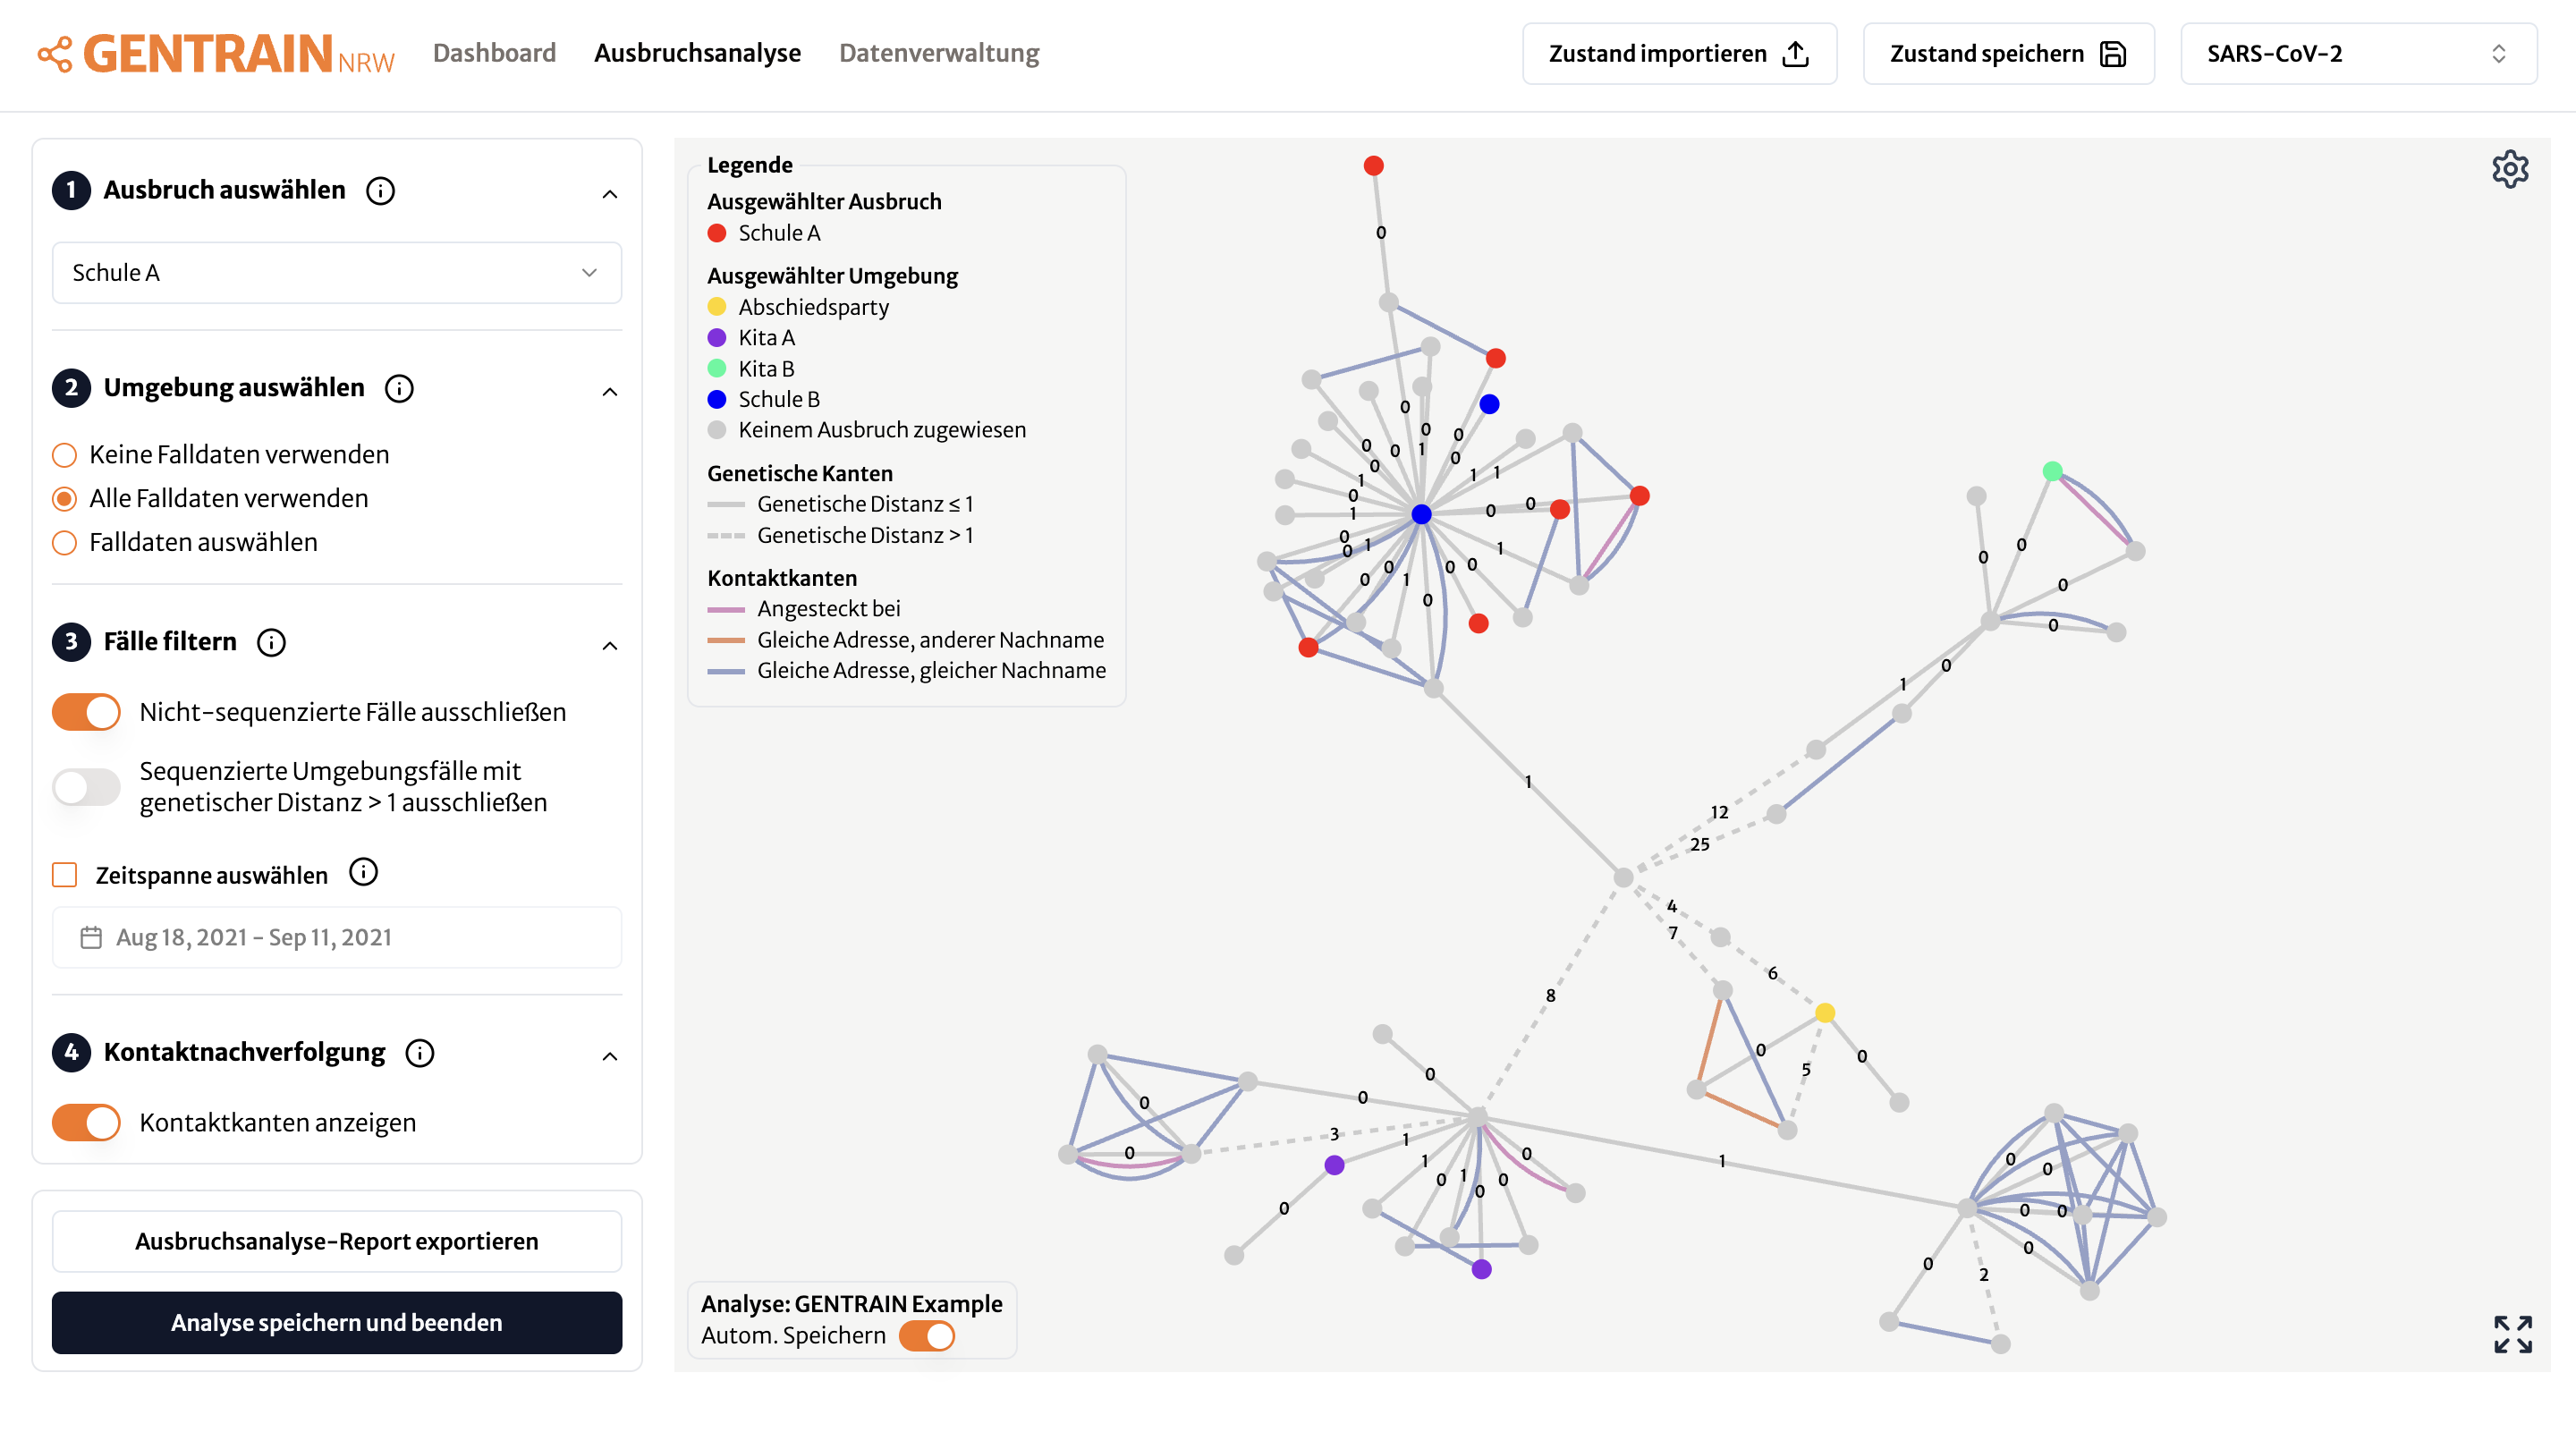
\includegraphics[width=\textwidth]{gentrain}
    \centering
    \caption[Disease outbreak analysis with GENTRAIN]{Disease outbreak analysis with GENTRAIN}
    \label{fig:gentrain}
\end{figure}

GENTRAIN operates within a web browser, where most processes are executed on the client side and data are stored in the local database of the web browser. Initially, the application analyzes imported sequences in terms of the mutations contained (see Section \ref{sec:nextclade}) and persists the results in the local database. This mutation information is a compact representation of the genome sequences and the obligatory information necessary for calculating genetic distance.
The genetic distances between all the sequences imported into the application are calculated based on the detected mutations (see Section \ref{sec:calculation_of_genetic_distances}). Subsequently, the genetic distances are stored in the local database, allowing the generation of an \acrshort{mst} to visualize the outbreak dynamics between the imported sequences. This \acrshort{mst}, which is based on genetics, is extended by contact edges, which represent contact tracing data imported by local public health authorities.
Figure \ref{fig:gentrain} provides a sneak peek at the application. It shows the procedure of a disease outbreak analysis, with genetic distance edges colored gray and contact edges colored differently.

\subsubsection{Nextclade Mutation Calling}
\label{sec:nextclade}
To retrieve mutation information from viral genome sequences, GENTRAIN uses Nextclade, which is a \acrfull{cli} developed by the Nextstrain project. The goal of the project is "to aid epidemiological understanding of pathogen spread and evolution and improve outbreak response" \cite{Nex2}. This section provides a detailed explanation of the Nextclade \acrfull{cli} pipeline with the ultimate goal of understanding how aligned mutation information is obtained from genome sequences. Only the steps relevant to this work are considered.

\begin{description}
    \item[Sequence alignment] The first stage of the pipeline aims to align input sequences, or query sequences, with a specified reference genome pair by pair. Small fragments are identified in which the queries and the reference match exactly. The estimated shift of a query sequence relative to the reference and the number of indels are determined from seed chains that cover sufficient regions of the query sequences. Combining all the resulting estimates produces a sequence of variable length that, with a high probability, covers the entire alignment \cite{Nex3}. The \acrshort{iupac} symbol for gaps is used to mark deleted nucleotides within aligned query sequences \cite{Nex5}. Insertions detected during the alignment are extracted into a separate file for mutation calling later on. If a query sequence is shorter than 100 nucleotides, the alignment is unreliable. Additionally, if a sequence diverges too much from the reference, the alignment may fail because a low number of similar fragments found. Reasons for this include the usage of an inappropriate reference, very low quality query sequences, or query sequences that are too short compared to the reference \cite{Nex3}.
    \item[Mutation calling] The positions at which the query and reference nucleotide sequences differ are identified. Depending on the type of mutation, different notation patterns are applied. For \acrshortpl{snv} the original nucleotide, the reference position and the new nucleotide are reported. For example, a mutation from adenine (\lstinline|A|) to guanine (\lstinline|G|) at reference position \lstinline|300| would be reported as \lstinline|A300G|. Insertions are extracted from the separate file created during sequence alignment. An insertion of the nucleotides \lstinline|ACT| after the reference position \lstinline|22030| would be annotated as \lstinline|22030:ACT|. Deleted regions inside the aligned query sequences are annotated as numeric ranges or reference positions for single nucleotide deletions. A single nucleotide deletion at the reference position \lstinline|300| would be identified as \lstinline|300-301| and a deletion ranging from the reference positions \lstinline|600| to \lstinline|605| would be identified as \lstinline|600-606| \cite{Nex5}. Ambiguous symbols in the \acrshort{iupac} nomenclature are handled differently. The \acrshort{iupac} symbol N is treated like deletions, which means that numerical ranges are specified. Therefore, a series of Ns ranging from the reference positions \lstinline|200| to \lstinline|209| would be annotated as \lstinline|200-210|. All other \acrshort{iupac} symbols, referred to as non-ACGTNs, are reported using both the symbol and the reference position. For example, a \lstinline|Y| at the reference position \lstinline|20021| would result in \lstinline{Y:20021} \cite{Nex5}. Nextclade \acrshort{cli} also counts the number of occurrences of each type of mutation and includes them in the set of results.
    \item[Phylogenetic placement] Nextclade \acrshort{cli} places all query sequences on a phylogenetic tree. For each query sequence, the most similar node in the reference tree is determined based on the mutations in the query and the reference nodes of the reference tree \cite{Nex6}. The reference tree also contains clade annotations that will be used for the next stage of clade assignment.
    \item[Clade assignment] A clade is a group of related genomic sequences. Since the reference tree from the previous stage contains clade annotations, the clade of each query sequence can be determined by identifying the clade of the nearest reference node in the phylogenetic tree. Nextclade \acrshort{cli} includes the associated clade for each query sequence in the set of results \cite{Nex7}.
\end{description}

Nextclade \acrshort{cli} was developed and optimized for large-scale analysis. \cite{Nex1} Although no benchmarking information was found from the Nextstrain project, an yet unpublished article by Ort et al. evaluated the Nextclade CLI runtime for different quantities of avian influenza virus genome sequences. The analysis of 100 sequences took about 0.7 seconds. In addition, Nextclade \acrshort{cli} processed 10,000 sequences in only 20 seconds, corresponding to a processing speed of 500 sequences per second. This allows for the assumption of linear scaling of the Nextclade \acrshort{cli} pipeline \cite{Ort1}.

Although it is only one step in the entire pipeline, subsequent sections will refer to the entire process as Nextclade mutation calling because the results of this step form the basis of the approaches carried out.

\subsubsection{Genetic Distance Calculation}
\label{sec:calculation_of_genetic_distances}
In order to extract differences between two genomes, a pairwise comparison of the sequenced nucleotides must be performed. The GENTRAIN application implements an algorithm originally developed by Alexander Dilthey and Jonas Weber to calculate the genetic distance between genomic sequences. The procedure consists of two phases. In the initial phase, two sequences are reconstructed and aligned with each other on the basis of the mutations detected for the sequence positions of the reference genome. In the subsequent stage, the genetic distance between these reconstructed sequences is incremented in a position-wise manner. This leads to a time complexity of $O(n)$ where n refers to the length of the reference genome. As two iterations are executed during the two phases, the algorithm has a constant factor of $2n$.

Based on the mutation information for each pair of sequences in the local database, both sequences are reconstructed taking into account the nucleotide shifts resulting from the indels. The result is two genome sequences of equal length with aligned nucleotide positions including genomic mutations. To obtain such sequences, the following pairwise nucleotide determination rules are applied for each position of the reference genome, based on the type of mutation present.
\begin{description}
  \item[\acrshort{snv}] The replacing nucleotide is added to the sequence that has an \acrshort{snv} at the current reference position. \acrshortpl{snv} also include ambiguous symbols from the \acrshort{iupac} nomenclature.
  \item[Insertion] The inserted nucleotides are appended to the sequences that have an insertion at the current reference position. In the event that both sequences contain an insertion at the current reference position, they are aligned against each other to identify the most significant overlap of both insertions. The PairwiseAligner of the Biopython package is utilized for the alignment process \cite{Bio1}. This package employs the Smith-Waterman algorithm, a widely recognized approach to find optimal alignments in genome sequences \cite{Bio2}. If one sequence has no insertion at the current position, the amount of inserted positions are filled with gaps.
  \item[Deletion] A gap is added to each sequence that has a deletion at the current reference position. If both sequences have a deletion, the reference position is skipped entirely.
  \item[No mutation] The reference nucleotide for the current position is added to the sequences that do not have a mutation at the current reference position.
\end{description}

Table \ref{table:exemplary_aligned_sequence_reconstruction_result} demonstrates this procedure based on a slice of two exemplary genome sequences. The example shows an ambiguous symbol at reference position 2, an insertion after reference position 3, and a missing symbol at reference position 7 for the first genome. The second genome has an \acrshort{snv} at reference position 5, and a deletion ranging from reference positions 8 to 10. It becomes also clear how sequences are aligned in the presence of indels.

\begin{table}[ht!]
    \caption{Exemplary pairwise sequence reconstruction}
    \centering
    \begin{tabular}{ l | c c c c c c c c c c c c } 
    & \textbf{1} & \textbf{2} & \textbf{3} & & & \textbf{4} & \textbf{5} & \textbf{6} & \textbf{7} & \textbf{8} & \textbf{9} & \textbf{10}\\
    \hline
    \textbf{Reference} & T & A & G & - & - & C & G & T & G & A & G & A \\
    \hline
    \textbf{First genome} & T & Y & G & G & A & C & G & T & N & A & G & A \\
    \hline
    \textbf{Second genome} & T & A & G & - & - & C & A & T & G & - & - & -\\
    \end{tabular}
    \label{table:exemplary_aligned_sequence_reconstruction_result}
\end{table}

Once both sequences were reconstructed and aligned, a genetic distance can be determined. Therefore, for each position where the sequences have a different nucleotide, the genetic distance is increased by 1. Because aligned sequences may be longer than the reference genome sequence, the positions in subsequent algorithmic steps are referred to as alignment positions. Since ambiguous symbols may represent the nucleotide of the other sequence, alignment positions with ambiguous symbols must be examined more closely. In addition, each indel increases the genetic distance by only 1, regardless of the number of nucleotides inserted or deleted. Therefore, the following rules apply, based on the \acrshort{iupac} symbol at the alignment position.

\begin{description}
  \item[Missing symbols] If one of the sequences has N at the current alignment position, the genetic distance is not increased to avoid false negatives.
  \item[Gaps] If a sequence has a gap at the current alignment position, the genetic distance increases only if this sequence had no gap at the previous alignment position.
  \item[Other ambiguous symbols] For other ambiguous symbols, the genetic distance is increased only if the symbol at the current alignment position cannot represent the nucleotide of the other sequence at the current alignment position.
\end{description}

Table \ref{table:exemplary_pairwise_distance_determination_result} shows the increase in the genetic distance between two already reconstructed and aligned sequences per alignment position. At alignment position 9, the genetic distance does not increase due to the presence of an N in the first genome. Since the ambiguous symbol Y cannot stand for nucleotide A according to the \acrshort{iupac} nomenclature, a difference is assumed at alignment position 2. Note that the genetic distance is increased by only 1 for both the insertion between alignment positions 4 and 5 in the first genome and the deletion ranging from alignment positions 10 to 12 in the second genome. 

\begin{table}[ht!]    
    \caption{Exemplary pairwise distance determination}
    \centering
    \begin{tabular}{ l | c c c c c c c c c c c c } 
    & \textbf{1} & \textbf{2} & \textbf{3} & \textbf{4} & \textbf{5} & \textbf{6} & \textbf{7} & \textbf{8} & \textbf{9} & \textbf{10} & \textbf{11} & \textbf{12} \\
    \hline
    \textbf{First genome} & T & Y & G & G & A & C & G & T & N & A & G & A \\
    \hline
    \textbf{Second genome} & T & A & G & - & - & C & A & T & G & - & - & - \\
     \hline
    \textbf{Genetic distance increase} & 0 & 1 & 0 & 1 & 0 & 0 & 1 & 0 & 0 & 1 & 0 & 0 \\
    \end{tabular}
    \label{table:exemplary_pairwise_distance_determination_result}
\end{table}

Sequenced genomes have the characteristic that the quality of sequencing at the beginning and end of the sequence is relatively low. To suppress the influence of these regions on the genetic distance, it is only increased if a specified number of proper symbols has been read from the beginning and the end of both sequences. The proper symbols are all \acrshort{iupac} symbols except Ns and gaps. Once the distances for all combinations of isolates have been calculated, they can be assembled into a distance matrix. Based on this genetic distance matrix, GENTRAIN generates an \acrshort{mst} visualization to facilitate the analysis of disease outbreaks.

\subsection{Related Work}
\label{cha:related_work}
In order to contribute to existing research, the current state of the art in efficient visualizations of large-scale viral outbreak dynamics was examined. 
First, applications designed to support outbreak analysis through user-oriented interfaces were identified. The Nextstrain project was already introduced in Section \ref{sec:nextclade} concerning the Nextclade \acrshort{cli}, which is used by GENTRAIN to identify mutations in genomes. In addition to the \acrshort{cli}, Nextstrain provides a user-oriented web application that visualizes outbreak dynamics based on genome sequences \cite{Nex9}. Like Nextclade \acrshort{cli}, the web application compares sequences against a reference genome. The relationships are then displayed using phylogenetic trees, which are also used by the Nextclade \acrshort{cli} to distinguish clades. However, the application crashed while processing 5,000 sequences, suggesting that it is not optimized for large-scale analysis. Microreact is another example of a user-oriented application that supports outbreak analysis. In an article, Argimón et al. described the motivations and underlying technical concepts behind the application \cite{Mic1}. The application allows users to visualize genome sequence relationships using different types of tree-based graphs, as trees are the most well-established tool for analyzing genomic dynamics. It was developed in response to the transition in genomics from sequencing a few representatives to sequencing large numbers of populations. This allows for more detailed analyses of highly similar genomes, which should be accessible to users with different levels of expertise. 
The authors also mentioned the challenges resulting from large-scale datasets. However, they addressed these issues by emphasizing the need for research on alternative visualizations for such scenarios. Therefore, in addition to using visualizations that represent seasonal and geographic contexts, the author proposed a "high-level clustering of tree branches with subsequent expansion of nodes of interest" \cite{Mic1}. It is also important to mention that Microreact only processes graphs that have already been constructed, and therefore does not calculate genetic distance matrices itself.

These applications focus on genetic-based outbreak analysis that also considers seasonal and geographic contexts. As described in Section \ref{sec:viral_outbreak_analysis}, genome sequence information can be used in a way to support traditional epidemiology, a procedure that was introduced as \acrshort{igs}. Walker et al. conducted research on the relationship between genome isolates and the potential of \acrshort{igs}, demonstrating the procedure using miscellaneous contact tracing and genetic data sets in urban scenarios \cite{Wal1}. The authors identified links between several independent outbreak scenarios, some of which crossed national borders.
Furthermore, Bludau et al. analyzed acceptance criteria and state of the art in the use of \acrshort{igs} by local public health authorities in Germany \cite{Blu1}. Their investigation showed that the degree to which different local public health authorities use \acrshort{igs} varies greatly. They emphasized the potential of \acrshort{igs} for disease surveillance by supporting outbreak analysis and investigation of transmission chains. It was also mentioned that the required sequence availability is highly dependent on the objectives of the local public health authorities. Retrospective analyses can be performed with a smaller number of available sequences, but real-time outbreak analyses require higher sequencing throughput. In general, the authors defined the goal of simultaneously improving access to genome analysis for non-specialists and expanding the genomic expertise of local public health authorities in Germany.
Furthermore, a paper by Hanke et al. discussed the potential of \acrshort{igs} for interrupting HIV transmission dynamics \cite{Han1}. The paper focused on the impact of crises such as the SARS-CoV-2 pandemic and the war in Ukraine, which has led to massive refugee movements. They predicted that a "full automation of laboratory and data analysis processes [...] will enable HIV-\acrshort{igs} to enhance efficiency, effectiveness and accuracy of the entire HIV operational workflow".

These findings on the relevance of \acrshort{igs} emphasizes the need for user-oriented applications that address \acrshort{igs}. They also highlight the necessity of making these applications capable of handling large-scale datasets, especially for retrospective analysis. Therefore, approaches for comparing genome sequences were explored, while focusing on their applicability to large-scale datasets.
First, sequence comparison should be separated into alignment-free and alignment-based approaches. The first group yields rapid results, while the latter focuses on achieving a higher accuracy \cite{Lei1}. One prominent method of representing genome sequences using alignment-free methods is the use of k-mers \cite{Lei1}. These are based on the frequencies of words consisting of nucleotide sequences and are comparable to n-grams, a concept widely used in natural language processing. However, since the GENTRAIN algorithm is based on the mutation information of genome sequences that were first aligned by the Nextclade \acrshort{cli}, this research focuses more on alignment-based sequence comparison. Applications such as GENTRAIN aim to extract very accurate distances from genome sequences because low distances are responsible for the identification of infection chains.

The Hamming distance indicates pairwise genetic distance by measuring the number of nucleotide differences between two aligned sequences \cite{Hos1}. Assuming error-free sequencing and no ambiguous symbols, this would strictly underestimate the distances calculated by GENTRAIN. In 2021, Grabowski and Kowalski published an article that addressed the quadratic scaling problem in Hamming distance matrices \cite{Gra1}. Therefore, the calculation of relevant Hamming distances was performed using variant methods to identify relevant candidates. Most of these methods identified relevant candidates by filtering out sequence pairs that exhibit a genetic distance of more than a specified distance threshold. In general, the algorithms applied showed about an order of magnitude faster than complete matrix calculations, demonstrating the potential for efficiency improvements in calculating selective genetic distance matrices.

Another procedure that has been widely explored in the field of genomic sequence comparison is \acrfull{anns}. The objective is to find nearest neighbors in high-dimensional datasets for which an accurate nearest neighbor search is no longer efficient while preserving accuracy to the greatest extent possible \cite{Wan1}. \acrshort{anns} algorithms can be categorized as graph-based, partition-based, quantization-based, and hash-based methods \cite{Wan1}. Each of these methods employs a distinct procedure to approximate the nearest neighbors. Partition-based \acrshort{anns} divides the high-dimensional space into multiple regions. Then, the nearest neighbors are searched in the region of the query or nearby regions \cite{Li1}. In quantization-based \acrshort{anns}, data vectors are divided into multiple subvectors to enable a more efficient search based on compact representations using the centroid indices identified for each subvector \cite{Pen1}. When using hash-based \acrshort{anns}, data are transformed into low-dimensional representations, called hashes, to efficiently identify similarities on a smaller scale \cite{Li1}. Graph-based \acrshort{anns} relies on the construction of a proximity graph, which is then traversed to find the closest nodes for a given query \cite{Wan1}.

In the field of genomic sequence comparison, hash-based \acrshort{anns} is widely used, while other ANNS categories are less represented in genomic sequence comparison. Several related studies have applied the so-called \acrfull{lsh} to identify similar genome sequences. Although the original purpose of hashing is to find hashes to minimize collisions, \acrshort{lsh} does the opposite. The observed inputs are sorted into so-called \acrshort{lsh} buckets, where the colliding hashes are placed in the same bucket. The OMH method \cite{Mar2}, developed by Marçais et al., approaches calculating the edit distance using unaligned sequences, while also taking the relative order of k-mers into account. This method achieves a low number of false negatives while reducing the required runtime. However, this work overcomes this challenge by using already aligned sequence information from Nextclade mutation calling. Other studies focusing on the identification of similar genome sequences in large-scale datasets aim to strike a balance between false positives and false negatives \cite{Mus1, Wan2}. Therefore, Nimrah Mustafa proposes an LSH approach based on an AND/OR construction of hash functions, where the OR component serves to reduce false negatives and the AND component serves to reduce false positives \cite{Mus1}. In 2024, Zhao et al. introduced the GSEARCH method that combines k-mer hashing of sequences with a graph-based \acrshort{anns} method to identify highly similar sequences in very large genome datasets \cite{Zha2}.
The genetic relatedness of the sequences was determined using the Jaccard distance exhibited from the hash representations of the sequences. Upon these distances an \acrshort{hnsw} (\acrlong{hnsw}) graph was constructed to avoid quadratic scaling of distance calculation. In an \acrshort{hnsw} graph, a query node is inserted by repeatedly comparing the query distance to a currently focused node with the distances to its neighboring nodes until the nearest neighbors of the query are found. This means that the query does not need to be compared to every node in the graph. To further improve time complexity, hierarchical levels are added to the graph, enabling a search to first be conducted within a coarser set of nodes before the degree of detail is incrementally being increased. This graph can be updated and expanded with new queries, thus avoiding the need to rebuild the graph. A more detailed explanation of the procedure can be found in the fundamental article on \acrshort{hnsw} graphs by Malkov and Yashunin \cite{Mal1}. GSEARCH exhibited a time complexity of $O(log n)$, overcoming the quadratic scaling of genetic distance matrices, and producing promising results for datasets comprising highly similar genomes \cite{Zha2}. Therefore, the application of \acrshort{hnsw} could be sufficient to compare genomes of the same virus, as in this work.

Several studies have been found on how to calculate genetic distances more efficiently and identify similar genomes in large datasets \cite{Gra1,Mar2,Zha2,Mus1}. However, a research gap has been identified regarding the effects of these optimizations on visualizations for outbreak analysis. Furthermore, current research primarily focuses on phylogenetic relations, representing a broader examination of lineages than the fine-grained analysis of direct infection chains. The latter forms the foundation for \acrshort{igs}, a topic that has been frequently discussed in research due to the SARS-CoV-2 pandemic, emphasizing its relevance in the near future \cite{Wal1, Wal2, Blu1, Han1}. User-oriented applications such as Nextstrain and Microreact partially cover \acrshort{igs} by combining genetic data with seasonal and geographic attributes. However, to the best of the authors' knowledge, GENTRAIN is the only user-oriented application that provides graph visualizations of traditional epidemiological connections, such as those collected by local public health authorities, as well as genetic relatedness.